\begingroup
\def\ThisCaption{Stationary relative-price response across recycling and supply conditions. Colour shows the analytical local derivative scaled by a ten-percentage-point increase in the gross asset-lending share at total originations of one. It is a linearised effect, not an exact finite-shock simulation. The black curve marks zero effect; dots identify the two configurations in Figure~\ref{fig:reallocation}. All points satisfy $\chi<1+\eta_R=2$. The output-supply reference is renormalised with $\rho$ to preserve unit reference prices.}
\ifdefined\SeparateArtwork
\par\addvspace{0.65\baselineskip}\noindent\begin{minipage}{\linewidth}
\captionsetup{type=figure}
\caption{\ThisCaption}
\label{fig:threshold}
\centering\small\itshape [Figure \thefigure\ near here]\par
\end{minipage}\par\addvspace{0.65\baselineskip}
\else
\begin{figure}[tbp]
\centering
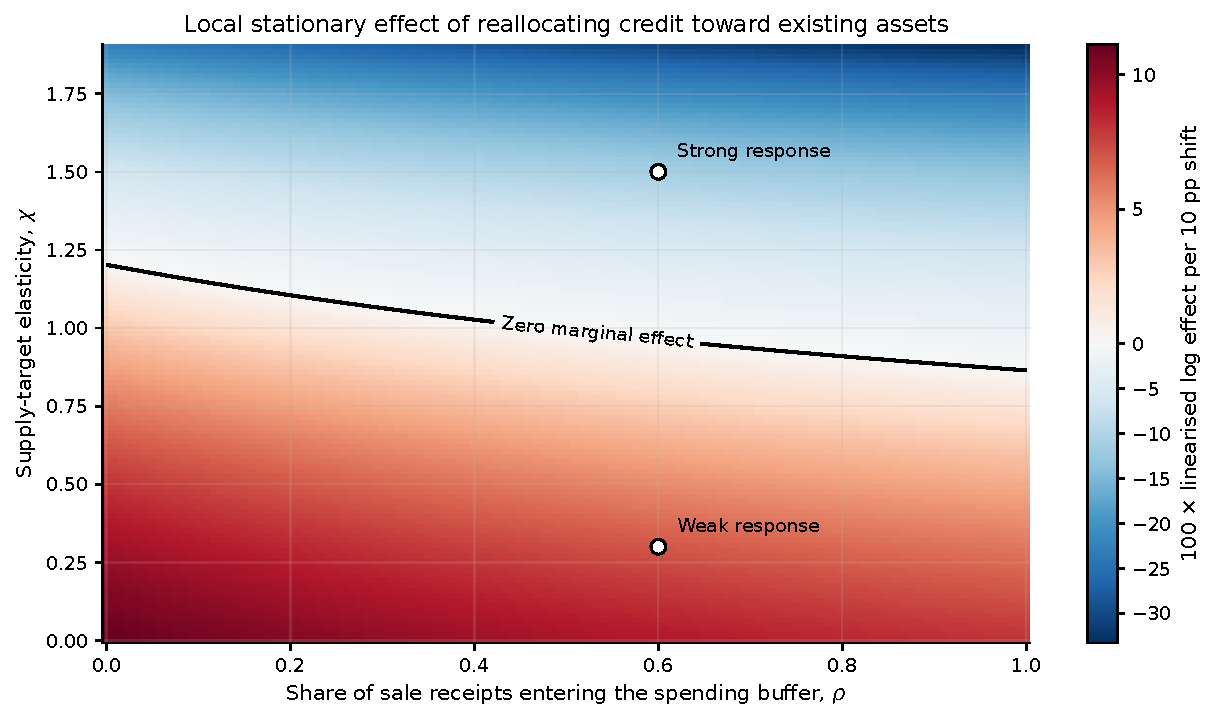
\includegraphics[width=\linewidth]{figures/fig03_threshold.pdf}
\caption{\ThisCaption}
\label{fig:threshold}
\end{figure}
\fi
\endgroup
